%----------------------------------------------------------------------------------------
%	PACKAGES AND THEMES
%----------------------------------------------------------------------------------------
\PassOptionsToPackage{table}{xcolor}
\documentclass[aspectratio=169,xcolor=dvipsnames,svgnames,x11names,fleqn]{beamer}
% \documentclass[aspectratio=169,xcolor=dvipsnames,fleqn]{beamer}

\usetheme{RedVelvet}

\usefonttheme[onlymath]{serif}
\newcommand{\showanswers}{yes}


\usepackage{xspace}
\usepackage{amsmath}
\usepackage{amssymb}
\usepackage{amsfonts}
\usepackage{color}
\usepackage{physics}
% \usepackage{mathbb}
\usepackage{rahul_math}
\usepackage{bigints}

\usepackage{graphicx} % Allows including images
\usepackage{booktabs} % Allows the use of \toprule, \midrule and \bottomrule in tables
\usepackage{tikz,pgfplots}

\usepackage{subfigure}
\usetikzlibrary{arrows}
\usepackage{minted}
\definecolor{LightGray}{gray}{0.9}
\definecolor{cream}{rgb}{0.92, 0.9, 0.55}
\definecolor{lightblue}{rgb}{0.68, 0.85, 0.9}


\usepackage{xcolor-material}
\usetikzlibrary{fit}
\usetikzlibrary{matrix}
\tikzset{%
apple/.pic={
    \fill [MaterialBrown] (-1/8,0)  arc (180:120:1 and 3/2) coordinate [pos=3/5] (@)-- ++(1/6,-1/7)  arc (120:180:5/4 and 3/2) -- cycle;
    \fill [MaterialLightGreen500] (0,-9/10)  .. controls ++(180:1/8) and ++(  0:1/4) .. (-1/3,  -1) .. controls ++(180:1/3) and ++(270:1/2) .. (  -1,   0) .. controls ++( 90:1/3) and ++(180:1/3) .. (-1/2, 3/4) .. controls ++(  0:1/8) and ++(135:1/8) .. (   0, 4/7)
    }
    }

\newcommand{\leftdoublequote}{\textcolor{blue}{\scalebox{3}{``}}}

\newcommand{\rightdoublequote}{\textcolor{blue}{\scalebox{3}{''}}}


\usepackage{textcomp}
\usepackage{fontawesome}
\usepackage{tikz,pgfplots}
\usetikzlibrary{shapes.callouts}
\usetikzlibrary{arrows}


\usepackage{overpic}

%----------------------------------------------------------------------------------------
%	TITLE PAGE
%----------------------------------------------------------------------------------------

\usepackage{tikz-qtree,tikz-qtree-compat}
\usetikzlibrary{tikzmark}
\usetikzlibrary{calc}


\title[CPE 486/586: Machine Learning]{CPE 486/586: Machine Learning for Engineers} % The short title appears at the bottom of every slide, the full title is only on the title page
\subtitle{09 Logistics Regression}

\author[Rahul Bhadani] {{\Large \textbf{Rahul Bhadani}}}

\institute[UAH] % Your institution as it will appear on the bottom of every slide, maybe shorthand to save space
{
    Electrical \& Computer Engineering,  The University of Alabama in Huntsville
}
\date

% \titlegraphic{
%    \includegraphics[width=0.4\linewidth]{figures/UAH_primary.png}
% }

\begin{document}

%-------------------------------------------------
\begin{frame}
    \titlepage
\end{frame}

%-------------------------------------------------
\begin{frame}{Outline}
    \backgroundtableofcontents
\end{frame}



 

\begin{frame}{First Thing First}
    
    \begin{center}
        \Large
        Logistics Regression is not a \textit{Regression} but a \textbf{classification} method.
    \end{center}
    
\end{frame}
%%%%%%%%%%%%%%%%%%%%%%%%%%%%%%%%%%%%%%%%%%%%%%%%%%%%%
\begin{sectionframe}{\faYelp}{Motivation}
\end{sectionframe}

%------------------------------------------------
\begin{frame}{Motivating Logistic Regression}

    \begin{itemize}
        \item Linear regression provides us a measure of how close a sample is to the decision boundary from the function $g(\x)$. That is the larger $|g(\x)|$ the farther a sample is from the plane. 
        \item Unfortunately, this score does not directly correspond to the probability that a sample belongs to a class. 
        \begin{itemize}
            \item We could try to think of a heuristic to connect $g(\x)$ to a probability; however, let us try to derive a relationship. 
            \item We need to revisit Bayes to get the conversation of logistic regression started.
        \end{itemize}
        \item Linear regression ended up having a very convenient solution (i.e., it was a convex optimization task) and we want to try to obtain a similar results -- {\em if possible}. 
    \end{itemize}
    
    
    \end{frame}
    
\begin{frame}{Goal}
    
    \Large
    \begin{center}
        Start with Bayes theorem to find a linear predictive model that can provide an estimate of the posterior probability.
    \end{center}
\end{frame}


%%%%%%%%%%%%%%%%%%%%%%%%%%%%%%%%%%%%%%%%%%%%%%%%%%%%%
\begin{sectionframe}{\faPieChart}{Revisiting Bayes' Theorem}
\end{sectionframe}


\begin{frame}{The Sum Rule in Probability}
    \begin{tblock}{}
        The marginal probability of a single random variable can be 
        obtained by summing (integrating) the probability density function 
        (pdf) over all values of all other variables. For example,
        \begin{multiequation}
            P(X) &= \sum_{Y\in\Ycal}P(X,Y) \\
            P(X) &= \sum_{Z\in\Zcal}\sum_{Y\in\Ycal}P(X,Y,Z)
            \end{multiequation}
    \end{tblock}
\end{frame}


%------------------------------------------------
\begin{frame}{The Product Rule in Probability}
    \begin{tblock}{}
    The joint probability can always be obtained by multiplying the  conditional probability (conditioned on one of the variables) with the  marginal probability of the conditioned variable
    \begin{multiequation}
    P(X, Y) = P(Y)P(X|Y) = P(X)P(Y|X)
    \end{multiequation}
    \end{tblock}
\end{frame}

%------------------------------------------------
\begin{frame}{Bayes' Rule}
    \begin{tblock}{}
    The combination of these two rules gives us Bayes Rule. Let $Y$ denote  the outcome that we seek to predict (e.g., healthy or not) and $X$  denote the variable(s) we are provided (e.g., medical records)

    \begin{multiequation}
    P(Y|X) = \frac{P(X|Y)P(Y)}{P(X)}
    = \frac{P(X|Y)P(Y)}{\sum_{y\in\Ycal}P(X, Y=y)}
    = \frac{P(X|Y)P(Y)}{\sum_{y\in\Ycal}P(X|Y=y)P(Y=y)}
    \end{multiequation}
    \end{tblock}
\end{frame}

\begin{frame}{Some Terminology in Bayes' Rule}

    In the context of 

    $$
    P(Y|X) = \frac{P(X|Y)P(Y)}{P(X)}
    $$

    \begin{itemize}
        \item $P(Y)$ is called \textbf{prior} distribution.
        \item $P(X|Y)$ is called the \textbf{likelihood}.
        \item $P(Y|X)$ is the posterior distribution.
        \item $P(X)$ is treated as constant for the known data and is marginal probability distribution. It can  be treated as a normalizing constant.
    \end{itemize}
\end{frame}

% https://www.stat.cmu.edu/~brian/463-663/week09/Chapter%2003.pdf
% https://web.stanford.edu/class/stats200/Lecture20.pdf
% https://sites.stat.columbia.edu/gelman/research/unpublished/prior_context_2.pdf
% https://courses.ucsf.edu/pluginfile.php/1666060/mod_resource/content/0/BayesLecture4.pdf
% https://www.stat.cmu.edu/~brian/463-663/week09/Chapter%2003.pdf
\begin{frame}{Bayesian Prior to Posterior}

    We could rewrite as

    \begin{tblockWing}{}
        \begin{center}
            \begin{multiequation}
                P(parameters|data) & = \cfrac{P(data|parameters)P(parameters)}{P(data)}\\
                posterior & \propto  normalized~~likelihood \times prior
            \end{multiequation}
        \end{center}
    \end{tblockWing}
    
\end{frame}

\begin{frame}{How to Get Prior}
    \begin{itemize}
        \item Past data: "today's posterior = tomorrow's prior"
        \item Meta-analysis of past data: amalgamation of multiple sources
        \item Expert knowledge
        \item Individual subjective opinion
    \end{itemize}
\end{frame}
\begin{frame}{Example: Bayes Rule for Email Classification}

    \begin{columns}
        \column{0.5\linewidth}

        \begin{center}
            {
                
\includegraphics[width=0.6\textwidth]{figures/spamemail.png}
            }
        \end{center}

        \column{0.5\linewidth}

        Consider $X \in \{0,1\}^W$, a vector of unique words, their value being ``0'' or ``1'' if the word appears in an email or not. This is known as a ``bag of words'' model.

    \end{columns}
\end{frame}

\begin{frame}{Example: Bayes Rule for Email Classification}

    We can write:

    \begin{multiequation}
  P(Y=\text{awesome}|Nigerian=1, Prince=1, Love=0, \ldots) \\= \frac{P(Y=\text{awesome})P(Nigerian=1, Prince=1, Love=0, \ldots|y)}{P(Nigerian=1, Prince=1, Love=0, \ldots)}
\end{multiequation}

Given our prior knowledge about the words ``Nigerian'' and ``Prince'' occurring in spam emails, it will be unlikely that this is an ``awesome'' email. 
    
\end{frame}

%------------------------------------------------
\begin{frame}{Making Decision with Bayes}
    Observation: $X$.

    \vspace{20pt}
    
    $\omega \in \Omega$: true class label.

    \vspace{10pt}
    
    $\omega^*$: class labels that we may predict using Bayes when we have the largest posterior probability.

\end{frame}

\begin{frame}{Selecting a Class using Bayes'}
    Formally, we have
    \begin{tblock}{}
        \begin{multiequation}
            \omega^* = \arg \max_{\omega \in \Omega} P(\omega |X)
            = \arg \max_{\omega \in \Omega} \frac{P(X|\omega)P(\omega)}{P(X)}
            = \arg \max_{\omega \in \Omega} P(X|\omega)P(\omega)
            \end{multiequation}
    \end{tblock}
where $P(X)$ can be omitted since it only acts as a normalization constant.

$\argmax$ is the argument of maxima which means the value $\omega$ at which $P(X|\omega)P(\omega)$ is the maximum.
\end{frame}

%------------------------------------------------
\begin{frame}{Visualizing the Posterior and Likelihood}
    \begin{center}
    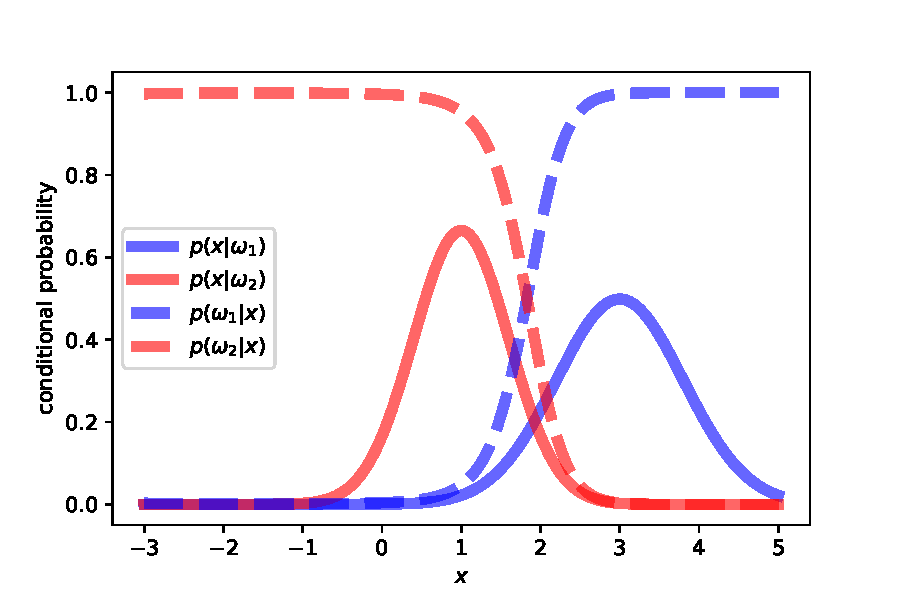
\includegraphics[width=.6\textwidth]{figures/bayes-post-likeli.pdf}
    \end{center}
\end{frame}
    

%------------------------------------------------
\begin{frame}{Probability of Error}
    \begin{center}
    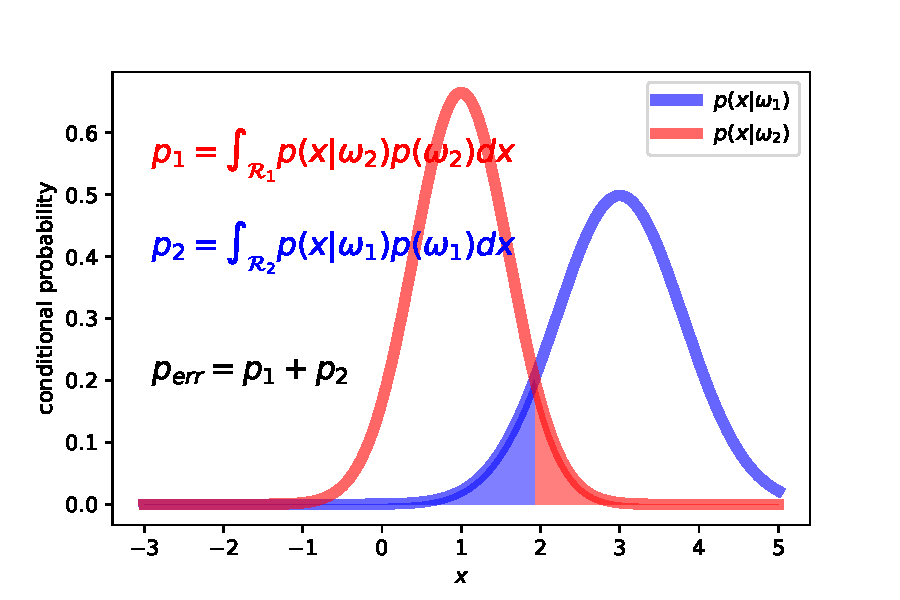
\includegraphics[width=.45\textwidth]{figures/bayes-likeli.pdf}
    \end{center}
    
    \begin{facts}{}
        Bayes has the minimum probability of error for any classifier of a random outcome. We write probability of error as
        \begin{multiequation}
            P(\textrm{error} | \xbf) = 1 - P(\omega^* | \xbf)
        \end{multiequation}
    \end{facts}
\end{frame}
    


%------------------------------------------------
\begin{frame}{Decision Making with Bayes}

    \begin{itemize}
        \item The Bayes decision rule (i.e., choose the outcome with the largest posterior) leads to the smallest probability of error. 
        \item Sometimes it is easier to work with the $\log$ of the posterior for numerical reasons and it leads to the same outcome since the $\log$ is a monotonically increasing function 
        \item {\bf Question}: If the Bayes decision rule has the smallest probability of error, why do we need machine learning? 
    \end{itemize}
    
\end{frame}

%------------------------------------------------
\begin{frame}{Why do we need ML if we have Bayes?}
    \begin{itemize}
    \item It is true that Bayes rule leads to the smallest probability of error; however, for this to be the case then we need to have access to $P(Y)$ and $P(X|Y)$. Or we need a very good estimate. 
    \begin{itemize}
        \item In reality, estimating these quantities can be very challenging -- or impossible -- with (1) making some assumptions or (2) a LOT of data.
        \item Example: Assume the data are Gaussian then estimate $\mu$ and $\Sigma$? 
        How much data do we need to estimate these parameters? What if the data are not Gaussian?
    \end{itemize}
    \item In practice, we need to make assumptions and learn to deal with limited data. 
    \end{itemize}
    
 
\end{frame}
    

\begin{frame}{}
        \begin{center}
            
\includegraphics[width=1.0\textwidth]{figures/bayes-mlhipster.png}
            \end{center}
\end{frame}
%------------------------------------------------
\begin{frame}{Na\"ive Bayes}

    \begin{tblock}{The Na\"ive Bayes Approach}
    Bayes rules states that we choose the class based on $p(\x|Y)P(Y)$, but estimating $p(\x|Y)P(Y)$ is {\em \color{MediumRed}very difficult}. So assume the features are conditionally independent! 
    \begin{multiequation}
    P(Y|\x) \propto p(\x|Y)P(Y)
    = p(x_1, \ldots, x_D|Y)P(Y)
    = P(Y) \prod_{j=1}^D p(x_j|Y)
    \end{multiequation}
    \begin{itemize}
    \item The advantage is that we need to estimate $D$ 1-dimensional distributions, not the $D$ dimensional joint distribution. 
    \item Is this assumption correct? Probably not, but it works well in many applications.
    \end{itemize}
    \end{tblock}
    
\end{frame}

\begin{sectionframe}{\faBraille}{Motivating Logistic Regression}
\end{sectionframe}


    %------------------------------------------------
\begin{frame}{A Dataset with Two Classes}
    \begin{columns}
        \column{0.5\linewidth}
        Consider the dataset given in the table:
    
        \begin{tabular}{|c|c|c|c|c|c|c|c|c|c|c|c|c|}
        \hline
        \textbf{x} & 1 & 2 & 3 & 4 & 5 & 6 & 7 & 8 & 9 & 10 & 11 & 12 \\
        \hline
        \textbf{y} & 1 & 0 & 0 & 0 & 0 & 1 & 1 & 1 & 1 & 1 & 1 & 0 \\
        \hline
        \end{tabular}
        A scatter plot for this dataset
        \column{0.5\linewidth}

    
        \begin{center}
            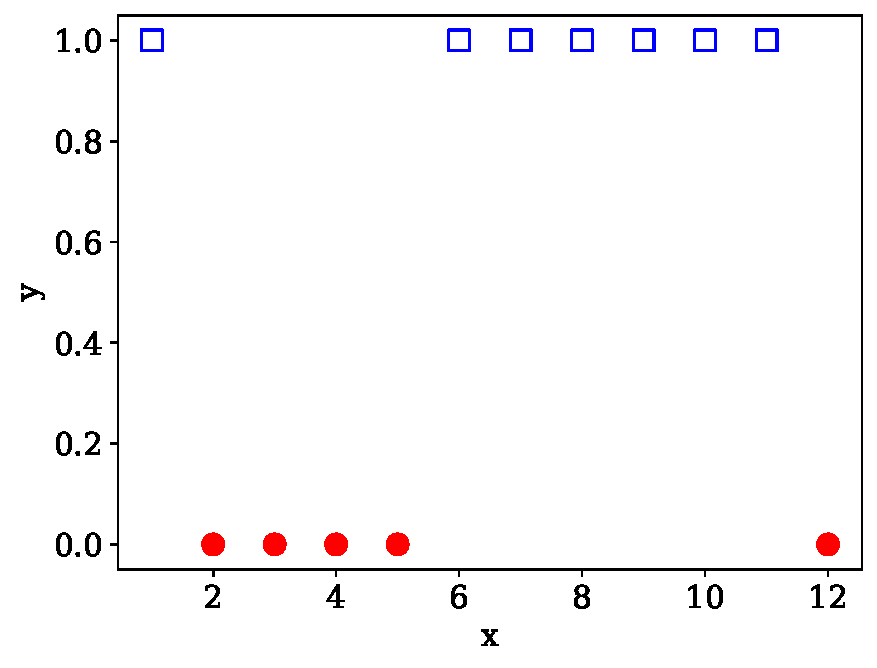
\includegraphics[width=1.0\textwidth]{figures/scatterplot_logistics_sample_data.pdf}
        \end{center}
    \end{columns}
\end{frame}
    
\begin{frame}{}
        \begin{center}
        \Large
            Clearly, distinguishing red and blue points won't work if we use the Linear Regression method. Also, linear regression predicts a continuous value, hence it won't be able to predict either 0 or 1.
        \end{center}
\end{frame}

%------------------------------------------------
\begin{frame}{Sigmoid Function}

    \begin{columns}
        \column{0.5\linewidth}
        By looking at the data, we think we can classify or correctly label the data points if we have a function that is low (0) for some low values of $x$, and high (1) for some values of $x$.
        One such function is \textbf{Sigmoid Function} or \textbf{Logistics Function} ($g(z)$ in the graph).
        $$
        g(z) = \cfrac{1}{1 + e^{-z}}
        $$
        \column{0.5\linewidth}
        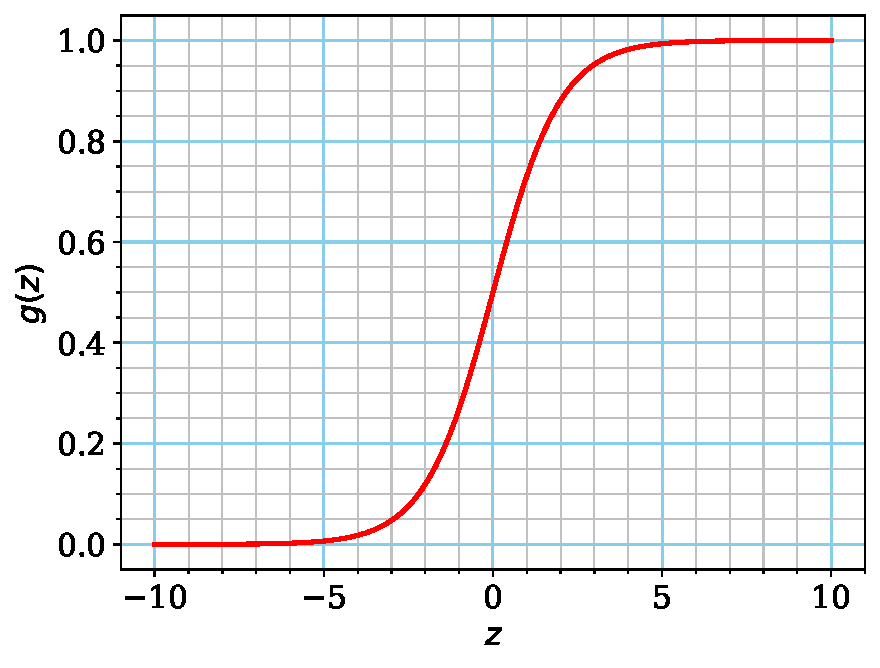
\includegraphics[width=0.88\textwidth]{figures/ssigmoid_function.pdf}
    \end{columns}    
\end{frame}

\begin{frame}{Sigmoid Function}
    We see that
    
    \begin{multiequation}
    \lim_{z\to-\infty} g(z) = 0
    \end{multiequation}
    
    and 
    
    \begin{multiequation}
    \lim_{z\to\infty} g(z) = 1
    \end{multiequation}
    
    It means, that for a very high positive value of $x$, the function approaches $1$, and for a very high negative value of $x$, the function approaches $0$.
\end{frame}

%------------------------------------------------
\begin{frame}{Generalized Sigmoid Function}
    Now, what if we want the slope to change faster or slower? How should we modify the Sigmoid function?
    
    \begin{columns}
    
        \column{.6\textwidth}
    
            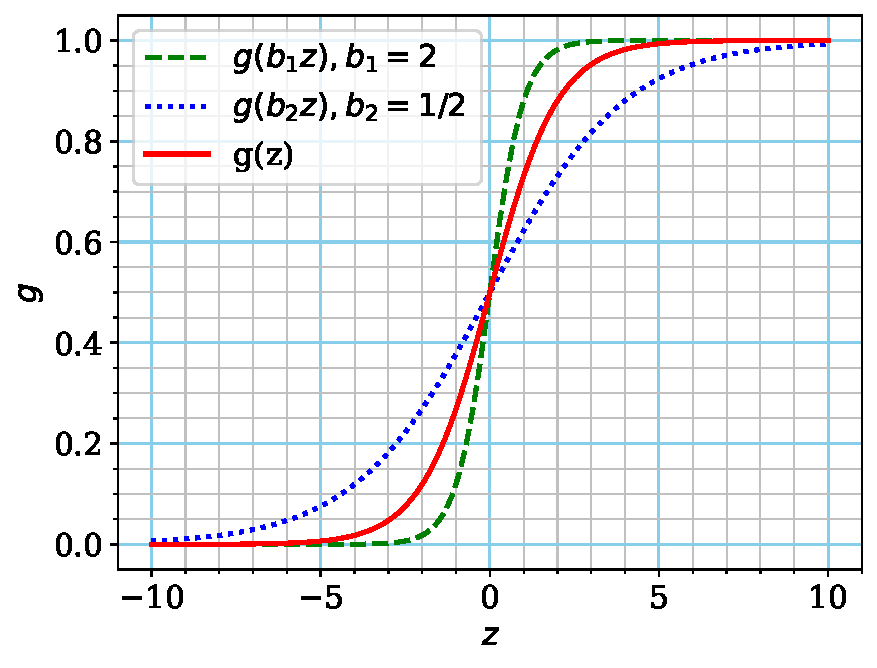
\includegraphics[width=0.7\textwidth]{figures/sigmoid_function_varying_slope.pdf}
        \column{.4\textwidth}
        
    $$
    g(z) = \cfrac{1}{1 + e^{-z\cdot b}}
    $$
    \end{columns}
    
\end{frame}
    
%------------------------------------------------
\begin{frame}{Defining Sigmoid Function for Logistics Regression}

    In the above example $b_1$, $b_2$ and $\pm a$ are learnable parameters that we are going to learn from data the same way we learned $w_1$ and $w_0$ in the linear regression.
    Thus, we consider a parameter vector $\boldsymbol{\theta}$ that consists of a vector of parameters to be learned using data $\textbf{x}$ that we can use to write a generalized version of sigmoid that is data-dependent by setting $z = \boldsymbol{\theta}^\top\textbf{x} $
    
    $$
    h_{\boldsymbol{\theta}}(\textbf{x}) = g(\boldsymbol{\theta}^\top\textbf{x} ) = \cfrac{1}{1 + e^{-\boldsymbol{\theta}^\top\textbf{x}}}
    $$
    
    
\end{frame}

%%%%%%%%%%%%%%%%%%%%%%%%%%%%%%%%%%%%%%%%%%%%%%%%%%%%%
\begin{sectionframe}{\faBullseye}{Logistics Regression}
\end{sectionframe}

\begin{frame}{Problem Statement in Logistics Regression}
    \begin{tblock}{}
        The overall goal in Logistics Regression becomes finding $P(Y|X)$, i.e, given information about the random variable $X$ that gives the distribution of the predictor variable, find the probability that the random variable $Y$  takes a certain value.
    \end{tblock}
\end{frame}

\begin{frame}{Assumptions in Logistics Regresions}
    
    \begin{itemize}
        \item \textbf{Linearity:} The model assumes that the relationship between the natural log of the probabilities (of each outcome and your predictor variable is linear.
        \item \textbf{No Outliers:} Logistics regression is very sensitive to outliers.
        \item \textbf{Independence:} Each observation point should be independent of each other.
    \end{itemize}
\end{frame}

%------------------------------------------------
\begin{frame}{Logistic Regression}

    \begin{tblock}{}
    
    
    From the earlier formulation, $h_{\boldsymbol{\theta}}$ estimates the probability that the data points belong $Y = 1$, and hence we can write it as
    
    \begin{multiequation}
        P(Y = 1 | X = x) = h_{\boldsymbol{\theta}}(\textbf{x}) 
    \end{multiequation}
    
    \begin{multiequation}
    P(Y = 0 | X = x) = 1-  h_{\boldsymbol{\theta}}(\textbf{x})
\end{multiequation}
    \end{tblock}
    
    \end{frame}


%------------------------------------------------
\begin{frame}{Cost Function}

    Just like linear regression, we need a cost function based on which we want to estimate $\boldsymbol{\theta}$.
    
    Here, we have two scenarios:
    
    \begin{enumerate}
        \item $y_i = 1$:
        \begin{itemize}
            \item if $h_{\boldsymbol{\theta}}(\textbf{x})  \approx 1$, cost $\approx 0$ (no penalty)
            \item if $h_{\boldsymbol{\theta}}(\textbf{x})  \approx 0$, cost $\approx$ very high
        \end{itemize}
    
        \item $y_i = 0$:
        \begin{itemize}
            \item if $h_{\boldsymbol{\theta}}(\textbf{x})  \approx 1$, cost $\approx $ very high
            \item if $h_{\boldsymbol{\theta}}(\textbf{x})  \approx 0$, cost $\approx 0$ (no penalty)
        \end{itemize}
    \end{enumerate}
    
    
    Then as the outcome is 0 or 1, it follows the Bernoulli Distribution.
    
    
\end{frame}

%------------------------------------------------
\begin{frame}{Bernoulli Distribution Revisited}
    \begin{facts}{}
        The Bernoulli distribution is a special case of the binomial distribution where a single trial is conducted (so $n$ would be $1$ for such a binomial distribution).
    \end{facts}
    
    
        The formula for pmf associated with a Bernoulli random variable over possible outcomes $x$ is given as follows:
    
    \begin{multiequation}
    f(x; p) =  \begin{cases} p &\quad \textrm{~if~} x= 1 \\ 1- p &\quad \textrm{~if~} x= 0 \end{cases}
\end{multiequation}
    We can also express this formula as,
    
\begin{multiequation}
    f(x, p) = p^x(1 - p)^{1 - x},\quad x \in \{0, 1\}
\end{multiequation}
    
\end{frame}

%------------------------------------------------
\begin{frame}{Likelihood Function}
    Hence, probability of assigning a label $y$ based on the data $\mathbf{x}$ is given by

\begin{multiequation}
P(Y = y| X = \mathbf{x}) =  h_{\boldsymbol{\theta}}(\textbf{x})^y \bigg[ 1 - h_{\boldsymbol{\theta}}(\textbf{x}) \bigg]^{(1-y)}
\end{multiequation}

Now, we write taking all data into account (all data points are independent):

\begin{multiequation}
L(\theta) = \Pi_{i=1}^n P(Y = y_i| X = \mathbf{x}_i) = \Pi_{i=1}^n h_{\boldsymbol{\theta}}(\textbf{x}_i)^{y_i} \bigg[ 1 - h_{\boldsymbol{\theta}}(\textbf{x}_i) \bigg]^{(1-y_i)}
\end{multiequation}

This is called \textbf{likelihood function}.

\end{frame}


%------------------------------------------------
\begin{frame}{Log-Likelihood Function}
    Now, take the log of the likelihood function, which is called the log-likelihood function:
\begin{multiequation}
    LL(\boldsymbol{\theta}) = \sum_{i=1}^n y_i \log ({ h_{\boldsymbol{\theta}}(\textbf{x}_i) }) + (1-y_i)\log \bigg[ 1 - h_{\boldsymbol{\theta}}(\textbf{x}_i) \bigg]
\end{multiequation}
    
    This is also called \textbf{cross-entropy loss}.
\end{frame}

\begin{frame}{Optimization Function}
    In the logistics regression, our goal becomes maximizing the log-likelihood by choosing the appropriate $\boldsymbol{\theta}$.
    For this, we take the partial derivative of $LL(\theta)$ with respect to  $\boldsymbol{\theta}$.
    

\end{frame}

\begin{frame}{Deriving the Optimization Function}
    Derive the expression for 
    
    \begin{multiequation}
    \cfrac{\partial LL(\boldsymbol{\theta})}{\partial \theta_j}
    \end{multiequation}
    for $j-th$ component of $\boldsymbol{\theta}$.
    
\end{frame}

\begin{frame}{Deriving the Optimization Function}

{\color{gray}Class work}

\end{frame}

\begin{frame}{Deriving the Optimization Function}

    {\color{gray}Class work}
    
\end{frame}

\begin{frame}{Deriving the Optimization Function}

    {\color{gray}Class work}
    
\end{frame}
    
\begin{frame}{Optimization Function}
    \begin{multiequation}
    \cfrac{\partial LL(\boldsymbol{\theta})}{\partial \theta_j} = \sum_{i=1}^n \bigg[ y_i - h_{\boldsymbol{\theta}}(\textbf{x}_i) \bigg]x_{ij}
    \end{multiequation}
    
    The derivation comes from the fact that the logistics function has a special property:
    
    \begin{multiequation}
    \cfrac{\partial g(z) }{\partial z} = g(z)[ 1 - g(z)]
    \end{multiequation}
\end{frame}
    

\begin{frame}{Logistics Regression with SGD}

        Equating $$\cfrac{\partial LL(\boldsymbol{\theta})}{\partial \theta_j}  = 0$$will give optimal $\theta_j^*$. However, the expression doesn't have any closed form, so we resort to using numerical methods for solving the optimization, and hence, in this case, we use \textbf{Gradient Ascent Optimization} which is equivalent to minimizing the negative of the log-likelihood function, for which we can use already discussed \textbf{Gradient Descent Optimization}.
\end{frame}

\begin{frame}{Updated Rule}
    $$
\theta_j \leftarrow \theta_j - \eta \cfrac{\partial LL(\boldsymbol{\theta})}{\partial \theta_j} 
$$

$$
\theta_j \leftarrow \theta_j - \eta \sum_{i=1}^n \bigg[ y_i - h_{\boldsymbol{\theta}}(\textbf{x}_i) \bigg]x_{ij}
$$
\end{frame}


\begin{frame}{Pseudo Code}
        Logistic regression is quite easy to code up using stochastic gradient descent. You'll need an approach to determine when to stop training.
       

        \begin{itemize}
            \item {\bf Input}: $\Dcal := \{(\x_i, y_i)\}_{i=1}^n$, $\eta$, $T$
            \item {\bf Initialize}: $\boldsymbol{\theta} = 0$ and $\theta_0 = 0$ \hfill {\color{MediumRed} \% or initialize from $\Ncal(0, \sigma)$}
            \item {\color{MediumBlue}\bf for} $t = 1, \ldots, T$
            \begin{itemize}
                \item {\color{MediumBlue}\bf for} $j = 1, \ldots, n$
                \begin{itemize}
                    \item $i=\texttt{np.random.randint}(n)$
                    \item $\boldsymbol{\theta} = \boldsymbol{\theta} + \eta (y_i - g(\x_i))\x_i$
                    \item $\theta_0 = \theta_0 + \eta (y_i - g(\x_i))$
                \end{itemize}
                \item {\color{MediumBlue}\bf if }\texttt{CONVERGED}, STOP
            \end{itemize}
        \end{itemize}
\end{frame}

\begin{frame}{Stopping Criteria}
    \begin{tblock}{}
        \begin{multiequation}
        \left\| \boldsymbol{\theta}_{t+1}  - \boldsymbol{\theta}_t \right\|_2^2 \leq \epsilon, \text{ or }
        \texttt{CrossEntropy}(t) - \texttt{CrossEntropy}(t+1) \leq \epsilon
        \end{multiequation}
    \end{tblock}
\end{frame}

%------------------------------------------------
\begin{frame}{Logistic Regression Example}

    \begin{center}
        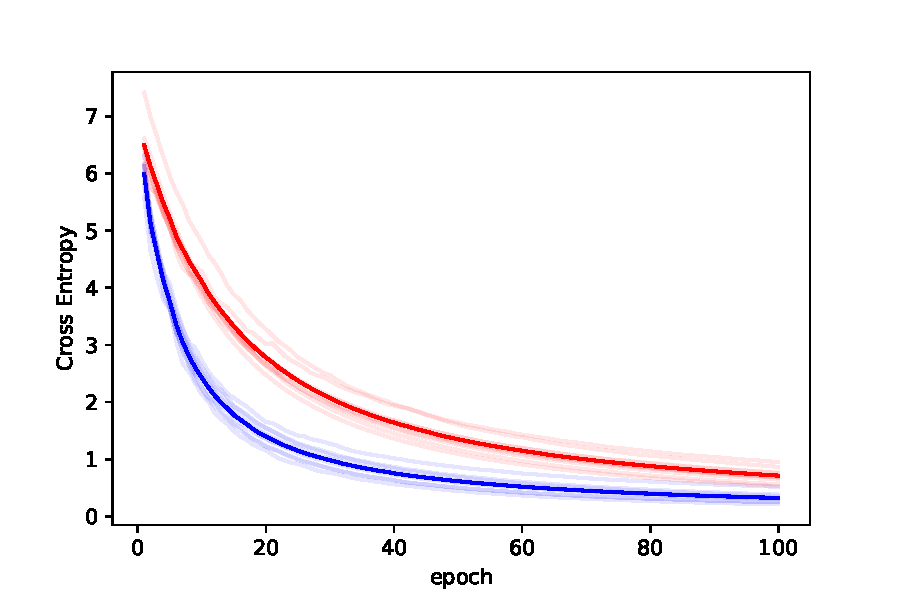
\includegraphics[width=.6\textwidth]{figures/lm-cross-entropy.pdf} \\
        {Cross entropy loss on the Iris dataset for two logistic regression models. The {\color{MediumBlue}blue} is trained with a learning rate of $\eta=0.0025$ and the {\color{MediumRed}red} is trained with a learning rate of $\eta=0.001$}
    \end{center}
    
\end{frame}
    
%------------------------------------------------
\begin{frame}{Logistic Regression Example}

    \begin{center}
        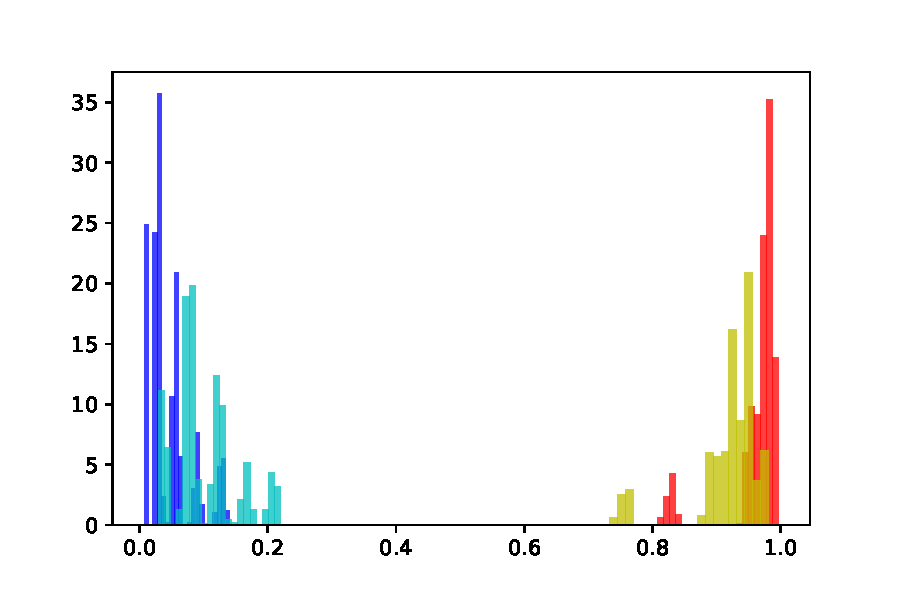
\includegraphics[width=.6\textwidth]{figures/lm-probs.pdf} \\
        Probabilities, $g(\x)$, on predicted data on a validation set. The Cyan/Yellow probabilities are from the model with $\eta=0.001$ and the Blue/Red probabilities are from the model with $\eta=0.0025$. 
    \end{center}
    
\end{frame}

%------------------------------------------------
\begin{frame}[containsverbatim]{Logistic Regression (in code)}

    \begin{minted}
        [
        framesep=1mm,
        baselinestretch=1.2,
        fontsize=\small
        ]
        {python}
    class LR: 
        def __init__(self, lr=0.0025, epochs=50, split=.1): 
            self.lr = lr 
            self.epochs = epochs 
            self.w = None 
            self.b = None 
            self.cross_ent = np.zeros(epochs)
            self.split = split
        
        def score(self, X): 
            return 1.0/(1 + np.exp(-(np.dot(self.w, X) + self.b)))
        
    \end{minted}
    
\end{frame}
    
%------------------------------------------------
\begin{frame}[containsverbatim]{Logistic Regression (in code)}

    \begin{minted}
        [
        framesep=1mm,
        baselinestretch=1.2,
        fontsize=\small
        ]
        {python}
        def crossent(self, X, y): 
            ce = np.log(self.score(X[y==1])).sum() + \
                     np.log(1.0 - self.score(X[y==0])).sum()
            return -ce
    \end{minted}
    
\end{frame}
    
    
    
    
    %------------------------------------------------
    \begin{frame}[containsverbatim]{Logistic Regression (in code)}
    
        \begin{minted}
            [
            framesep=1mm,
            baselinestretch=1.2,
            fontsize=\small
            ]
            {python}
        def fit(self, X, y): 
            i = np.random.permutation(len(y))
            X, y = X[i], y[i]
            self.w, self.b = np.zeros(X.shape[1]), 0
            M = np.floor((1-self.split)*len(y)).astype(int)
            Xtr, ytr, Xva, yva = X[:M], y[:M], X[M:], y[M:]        
            for t in range(self.epochs): 
                # run stochastic gradient descent
                for i in np.random.permutation(len(ytr)): 
                    self.w += self.lr*(ytr[i] - self.score(Xtr[i]))*Xtr[i]
                    self.b += self.lr*(ytr[i] - self.score(Xtr[i]))
                self.cross_ent[t] = self.crossent(Xva, yva)
            \end{minted}
    
    \end{frame}
    
    
    %------------------------------------------------
    \begin{frame}[containsverbatim]{Logistic Regression (in code)}
    
        \begin{minted}
            [
            framesep=1mm,
            baselinestretch=1.2,
            fontsize=\small
            ]
            {python}
        def predict(self, X): 
            return 1.0*(self.score(X[i]) >= 0.5)
        
        def predict_proba(self, X): 
            return self.score(X[i])
        
        def predict_log_proba(self, X): 
            return np.log(self.predict_proba(X))
        \end{minted}
    
\end{frame}
    
    
    %------------------------------------------------
\begin{frame}[containsverbatim]{Logistics Regression Using Sklearn}
    \begin{minted}
    [
    framesep=1mm,
    baselinestretch=1.2,
    fontsize=\small
    ]
    {python}
    import numpy as np
    from sklearn.linear_model import LogisticRegression
    
    # Create an instance of a Logistic Regression Classifier and fit the data.
    logreg = LogisticRegression()
    logreg.fit(x, y.ravel())
    
    # Predict
    y_hat = logreg.predict(x)
    
    print("Predictions:", y_hat)
    \end{minted}
        
\end{frame}
    
    
\begin{sectionframe}{\faPencilSquareO}{Logistic Regression Performance Evaluation}
\end{sectionframe}

\begin{frame}{Accuracy}
    Accuracy is a metric used to evaluate the performance of classification models. Informally, accuracy is the fraction of predictions our model got right. It measures the ratio of correctly predicted instances (true positives and true negatives) to the total number of instances.
    
    $$
    \text{Accuracy} = \frac{\text{Number of correct predictions}}{\text{Total number of predictions}}
    $$
    
\end{frame}

%------------------------------------------------
\begin{frame}[containsverbatim]{Confusion Matrix}
    Confusion Matrix displays how many of the data points were classified correctly and incorrectly.
    
    \begin{minted}
        [
        framesep=1mm,
        baselinestretch=1.2,
        fontsize=\small
        ]
        {python}
from sklearn.metrics import confusion_matrix
confusion_matrix = confusion_matrix(y, y_hat)
print(confusion_matrix)
    \end{minted}
\end{frame}


%------------------------------------------------
%------------------------------------------------
\begin{frame}{True Positive (tp)}
    \small
    \begin{columns}
        \column{0.5\textwidth}
        
\includegraphics[width=\textwidth]{figures/TP.pdf} % Placeholder image
        \column{0.5\textwidth}
        \begin{tblock}{}
            \textbf{True Positive (tp)}: Arpita has cancer. She takes a medical test for cancer, and the test result is positive. This is a true positive because the test correctly identified that Arpita has cancer.
        \end{tblock}
    \end{columns}
\end{frame}
    
    %------------------------------------------------
\begin{frame}{True Negative (tn)}
    \small
    \begin{columns}
        \column{0.5\textwidth}
        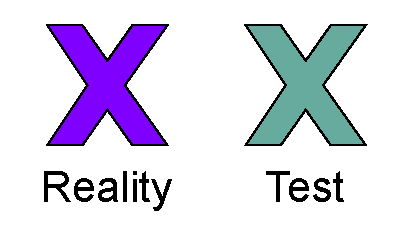
\includegraphics[width=\textwidth]{figures/TN.pdf} % Placeholder image
        \column{0.5\textwidth}
        \begin{tblock}{}
            \textbf{True Negative (tn)}: Mumtaj does not have cancer. She takes the same medical test, and the test result is negative. This is a true negative because the test correctly identified that Mumtaj does not have cancer.
        \end{tblock}
    \end{columns}
\end{frame}
    
    %------------------------------------------------
\begin{frame}{False Positive (fp)}
    \small
    \begin{columns}
        \column{0.5\textwidth}
        
\includegraphics[width=\textwidth]{figures/FP.pdf} % Placeholder image
        \column{0.5\textwidth}
        \begin{tblock}{}
            \textbf{False Positive (fp)}: Niu does not have cancer. However, when she takes the medical test, the test result is positive. This is a false positive because the test incorrectly identified that Niu has cancer.
        \end{tblock}
    \end{columns}
\end{frame}
    
    %------------------------------------------------
\begin{frame}{False Negative (fn)}
    \small
    \begin{columns}
        \column{0.5\textwidth}
        
\includegraphics[width=\textwidth]{figures/FN.pdf} % Placeholder image
        \column{0.5\textwidth}
        \begin{tblock}{}
            \textbf{False Negative (fn)}: Diana has cancer. However, when she takes the medical test, the test result is negative. This is a false negative because the test incorrectly identified that Diana does not have cancer.
        \end{tblock}
    \end{columns}
\end{frame}


\begin{frame}{}
    \begin{center}
        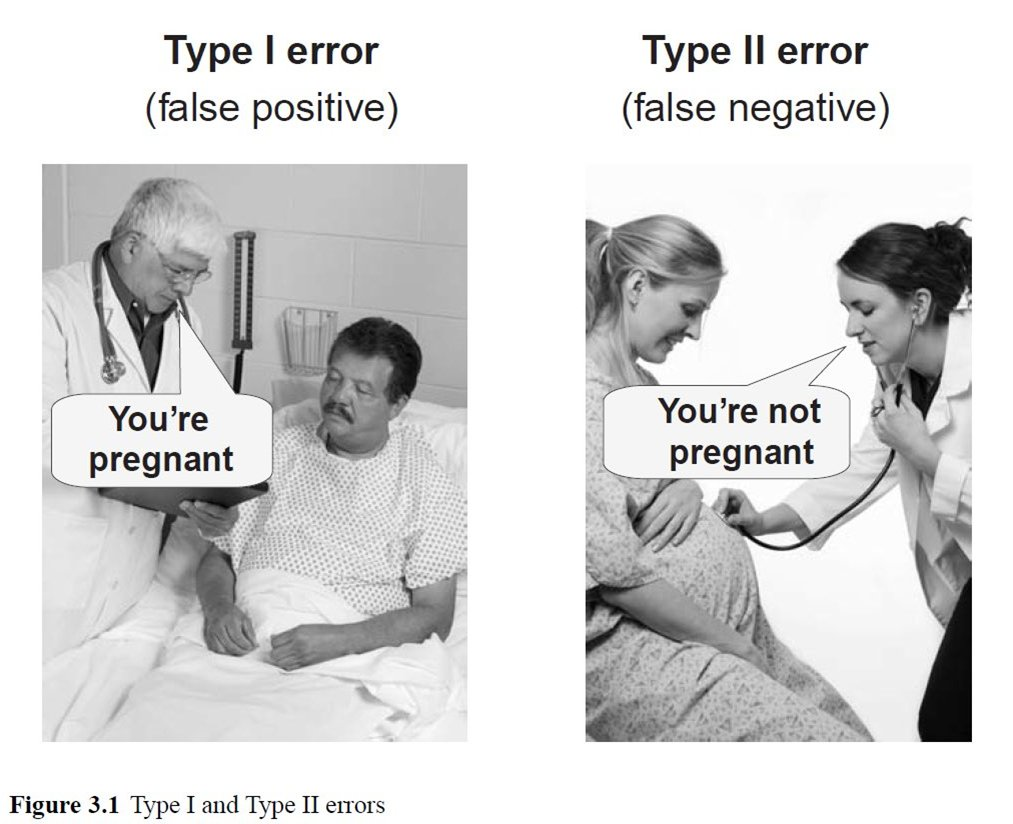
\includegraphics[width=0.65\textwidth]{figures/typeI_typeII.jpeg}
    \end{center}
\end{frame}
    
\begin{frame}{Precision}

\textbf{Precision} is the ratio

$$
\textrm{Precision} = \cfrac{tp}{tp + fp}
$$
This means the classifier cannot label a sample as positive if it is negative.
\end{frame}

\begin{frame}{Recall}
    \textbf{Recall} is

$$
\textrm{Recall} = \cfrac{tp}{tp + fn}
$$
It is the ability of the classifier to find all the positive samples.

\end{frame}

\begin{frame}{F-Score}



    \textbf{F-score} is the weighted harmonic mean of the precision and recall.

$$
F_{score} = 2\times \cfrac{Precision \times Recall}{Precision + Recall}
$$
    
\end{frame}

\begin{frame}{Support}
    \textbf{Support} is the number of occurrences of each class in the test set.
\end{frame}

\begin{frame}[containsverbatim]{In Sklearn: ...}
    \begin{minted}
        [
        framesep=1mm,
        baselinestretch=1.2,
        fontsize=\normalsize
        ]
        {python}
        from sklearn.metrics import classification_report
        print(classification_report(y, y_hat))
        \end{minted}
    
\end{frame}

%------------------------------------------------
\begin{frame}[containsverbatim]{Receiver Operating Characteristic (ROC)}
    An ROC curve (receiver operating characteristic curve) is a graph showing the performance of a classification model at all classification thresholds (0.5 by default). This curve plots two parameters:
    
    \begin{itemize}
        \item True Positive Rate (TPR)
        \item False Positive Rate (FPR)
    \end{itemize}
    
    An ROC curve plots TPR vs. FPR at different classification thresholds. Lowering the classification threshold classifies more items as positive, thus increasing both False Positives and True Positives.

\end{frame}
    
%------------------------------------------------
\begin{frame}{Classification Threshold}

    \begin{tblock}{Definition}
        In binary classification, the threshold determines the decision boundary for predicted probabilities. If the probability is above the threshold, the observation is classified as positive class; below as negative class.
    \end{tblock}
    \begin{tblock}{Example}
        Logistic regression typically uses 0.5 as default threshold. Probabilities $\geq 0.5$ are classified as positive, $<0.5$ as negative.
    \end{tblock}

\end{frame}

%------------------------------------------------
\begin{frame}{Thresholds \& ROC Curves}

        \begin{tblock}{Threshold Variation}
            Each point on a ROC curve represents a different threshold (0-1). Lower thresholds increase both False Positives and True Positives.
        \end{tblock}
        \begin{tblock}{Optimal Threshold}
            Determined by balancing TP/FP tradeoff. Can be calculated directly from ROC curves or found through grid search, depending on misclassification costs.
        \end{tblock}
    \end{frame}
    

    %------------------------------------------------
\begin{frame}{AUC (Area Under the ROC Curve)}
        \begin{tblock}{Definition}
            Measures entire area under ROC curve (0-1). Probability that model ranks random positive example higher than random negative example.
        \end{tblock}
        \begin{tblock}{Interpretation}
            0.0 = 100\% wrong predictions\\
            1.0 = 100\% correct predictions
        \end{tblock}
        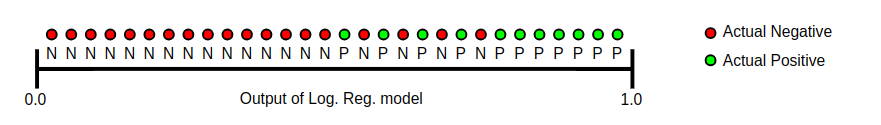
\includegraphics[width=0.8\textwidth]{figures/Logit_AUC_ROC.png}
\end{frame}

%------------------------------------------------
\begin{frame}[containsverbatim]{AUC Properties \& Caveats}
        \begin{tblock}{Advantages}
            \begin{itemize}
                \item Scale-invariant: Ranks predictions well
                \item Threshold-invariant: Evaluates all thresholds
            \end{itemize}
        \end{tblock}
        \begin{tblock}{Limitations}
            \begin{itemize}
                \item Doesn't assess calibrated probabilities
                \item Not suitable for cost-sensitive tasks
            \end{itemize}
        \end{tblock}
\end{frame}


\begin{frame}[containsverbatim]{AUC using Sklearn}
    \begin{minted}[fontsize=\small]{python}
        # Example from sklearn documentation
        from sklearn.metrics import roc_auc_score, roc_curve
        y = [1, 1, 0, 0]
        y_hat = [0.9, 0.6, 0.4, 0.2]
        print(roc_auc_score(y, y_hat))  # Output: 1.0
            \end{minted}
\end{frame}
    

\begin{frame}[containsverbatim]{ROC in Sklearn}
    \begin{minted}
        [
        framesep=1mm,
        baselinestretch=1.2,
        fontsize=\footnotesize
        ]
        {python}
        from sklearn.metrics import roc_auc_score
        from sklearn.metrics import roc_curve
        logit_roc_auc = roc_auc_score(y, y_hat)
        fpr, tpr, threshold = roc_curve(y, y_hat)
        
        plt.figure()
        plt.plot(fpr, tpr, 
            label='Logistics Reression (area = %0.2f)'% logit_roc_auc)
        plt.plot([0, 1], [0, 1], 'r--')
        plt.xlabel('False Positive Rate')
        plt.ylabel('True Positive Rate')
        plt.title('Receive Operating Characteristics (ROC) curve')
        plt.legend(loc='lower right')
        plt.show()
        \end{minted}
        
\end{frame}

\begin{frame}[containsverbatim]{ROC in Sklearn}

    \begin{center}
        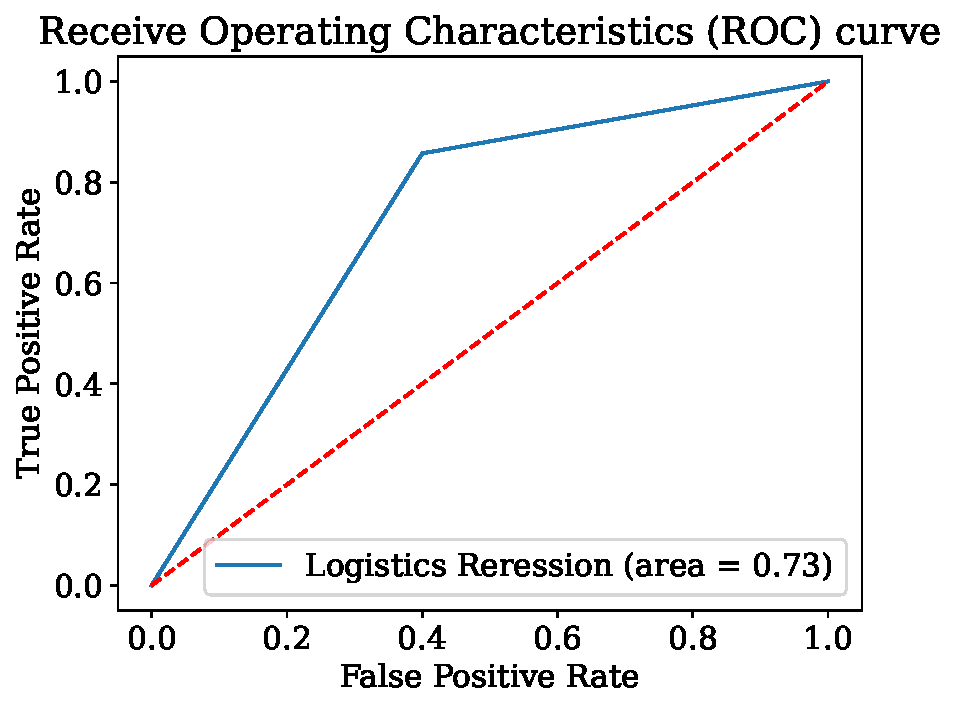
\includegraphics[width=0.49\textwidth]{figures/ROC_Curve.pdf}
    \end{center}
        
\end{frame}

\begin{sectionframe}{\faCopy~\faCopy}{Multi-Class Logistic Regression}
\end{sectionframe}


\begin{frame}{Multi-class}

    The binary logistic regression assumes that the label $y_i \in \{0, 1 \}$, while multi-class cases have more than two classes, i.e. , $y_i \in \{ 1, 2, \cdots, k\}$ where $k$ is the number of classes.

    \begin{itemize}
        \item In this case, we need to estimate the probability for each of the $K$ classes. 
    \end{itemize}
    
\end{frame}

\begin{frame}{Hypothessis in Multi-class}
    
    Multi-class hypothesis is written as 

    \begin{multiequation}
        h_{\boldsymbol{\theta}} = \begin{bmatrix}
            P( y = 1 | \xbf ; \boldsymbol{\theta})\\
            P( y = 2 | \xbf ; \boldsymbol{\theta})\\
            \cdots  \\
            P( y = k | \xbf ; \boldsymbol{\theta})
        \end{bmatrix}
    \end{multiequation}

    Assumption: no ordinal relationship between classes.

\end{frame}

\begin{frame}{Hypothessis in Multi-class}

    We will need one linear signal for each of the $k$ classes, which should be independent conditioned on $\xbf$.

    We compute $k$ linear signals by the dot product between the input x and $k$ independent weight vectors $\wbf_k$ as

    \begin{multiequation}
        \begin{bmatrix}
            \wbf_1^\top \xbf\\\wbf_2^\top \xbf\\\wbf_k^\top \xbf
        \end{bmatrix}
    \end{multiequation}

    Now, we need to map $k$ linear outputs to $k$ probability.
    
\end{frame}

\begin{frame}{Softmax Function}

    We need to use softmax function for generalized form the signmoid function which can be written as:

$$
    softmax(y_i) = \cfrac{\exp(y_i)}{\sum_{j=1}^n \exp (y_j)}
$$    
Softmax function gives the probability of each sample belonging to a certain class.

Thus, 

\begin{multiequation}
    h_{\boldsymbol{\theta}} = \cfrac{1}{\sum_{i = 1}^k \exp(\wbf_i^\top \xbf)} \begin{bmatrix}
        \exp(\wbf_1^\top \xbf) \\ \exp(\wbf_2^\top \xbf) \\ \cdots \\ \exp(\wbf_k^\top \xbf)
    \end{bmatrix}
\end{multiequation}
\end{frame}

\begin{frame}{Loss Function in Multi-class Logistics Regression}
    
    \begin{multiequation}
        L(\xbf_i, \ybf_i, \boldsymbol{\theta}) = -\sum_k \ybf_{ik} \log \hat{\ybf}_{ik} = -\sum_k \ybf_{ik} \log \bigg(\cfrac{\exp(\boldsymbol{\theta}_k^\top \xbf_i )}{\sum_{j}^k \exp(\boldsymbol{\theta}_j^\top \xbf_i )} \bigg)
    \end{multiequation}

    $y_i$ is one-hot encoding for labels, $\hat{\ybf}_i$ is the predicted distribution.

\end{frame}

\begin{frame}{One Hot Encoding for Multi-class Scenario}
    
    Consider four classes: $\{$Dog, Cat, Horse, Cheetah $\}$ that can be assigned numerals as $\{1, 2, 3, 4\}$. 

    In one hot-encoding, it can be written as:
    \begin{multiequation}
        \begin{bmatrix}
            1 & 0 & 0 & 0 & -- & Dog\\
            0 & 1 & 0 & 0 & -- & Cat\\
            0 & 0 & 1 & 0 & -- & Horse\\
            0 & 0 & 0 & 1 & -- & Cheetah
        \end{bmatrix}
    \end{multiequation}
\end{frame}

    
      %------------------------------------------------
    
    \begin{frame}[containsverbatim]{Python Notebook}
    \begin{center}
    \small
    { \color{Red}{\url{https://github.com/rahulbhadani/CPE486586_FA26/blob/master/Code/CPE486586_Ch09_Logistics_Regression.ipynb}}}
    \end{center}
    \end{frame}
    
    %------------------------------------------------
    
    \begin{frame}
        \Huge{\centerline{\color{MediumBlue}\textbf{The End}}}
    \end{frame}

\end{document}